\section{Anwendung: Wellenausbreitung auf einer Kugel oder der Tsunami von 2011}
Am 11.~M"arz 2011 l"oste ein Erdbeben der St"arke 9 im japanischen
Meer, das Sendai Erdbeben, einen Tsunami aus, der grosse K"ustengebiete
Japans verw"ustete, "uber
15000 Tote forderte und Unf"alle in mehreren Kernkraftwerken
ausl"oste, wovon der Unfall in Fukushima-Daichi mit einer
teilweisen Kernschmelze der schwerwiegendste war.
Tsunamis sind von Erdbeben ausgel"oste Wellen, die im offenen
Meer unscheinbar sind, aber wegen der mit kleiner werdender Wassertiefe
geringeren Ausbreitungsgeschwindigkeit in K"ustenn"ahe grosse
Amplituden erreichen k"onnen. Die Ausbreitung solcher Wellen
kann nat"urlich mit partiellen Differentialgleichungen modelliert
und berechnet werden. Die Abbildungen \ref{tsunamiausbreitung}
und \ref{tsunamienergie}
zeigt die mit einem Computer berechnete Ausbreitung des vom
Sendai-Erdbeben erzeugten Tsunami durch den Pazifik.
Dieses Modell ber"ucksichtigt offenbar die Topographie des
Meeresbodens.

Eine direkte Berechnung der Wellenausbreitung mit der bisher
gelernten Theorie ist nat"urlich nicht m"oglich, dazu m"usste
Topographie und K"ustenlinie des Pazifik im Detail bekannt
sein. Als vereinfachtes
Modell k"onnen wir jedoch versuchen, die Wellenausbreitung auf
einer Kugeloberfl"ache zu verstehen, dies entspricht einer 
kugelf"ormigen Erde, die mit einem Meer konstanter Tiefe bedeckt
ist.

\begin{figure}
\begin{center}
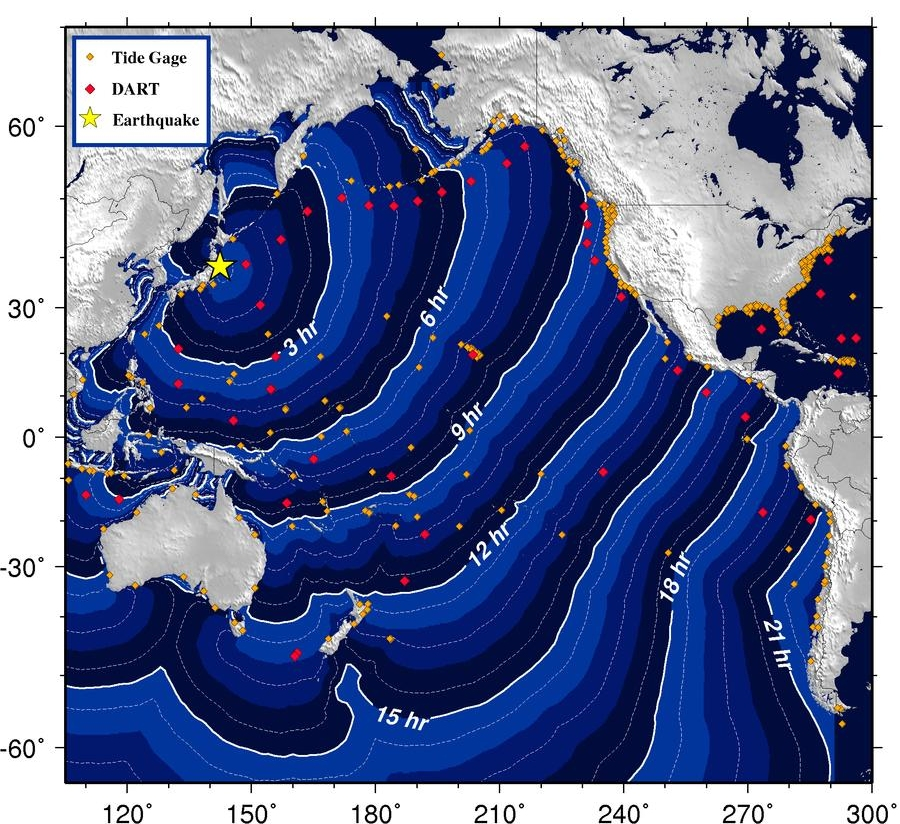
\includegraphics[width=\hsize]{graphics/sendainoaa}
\end{center}
\caption{Ausbreitung des vom Sendai-Erdbeben vom 11.~M"arz 2011 
ausgel"osten Tsunami durch den Pazifik nach einer Simulation der NOAA.
Hawai und andere Inseln reduzieren die Wassertiefe und damit die
Ausbreitungsgeschwindigkeit und verz"ogern damit die Ausbreitung
der Welle. Ebenfalls deutlich beobachtbar ist die Abschattung 
der Welle durch grosse Hindernisse wie Neuseeland.
\label{tsunamiausbreitung}}
\end{figure}

\begin{figure}
\begin{center}
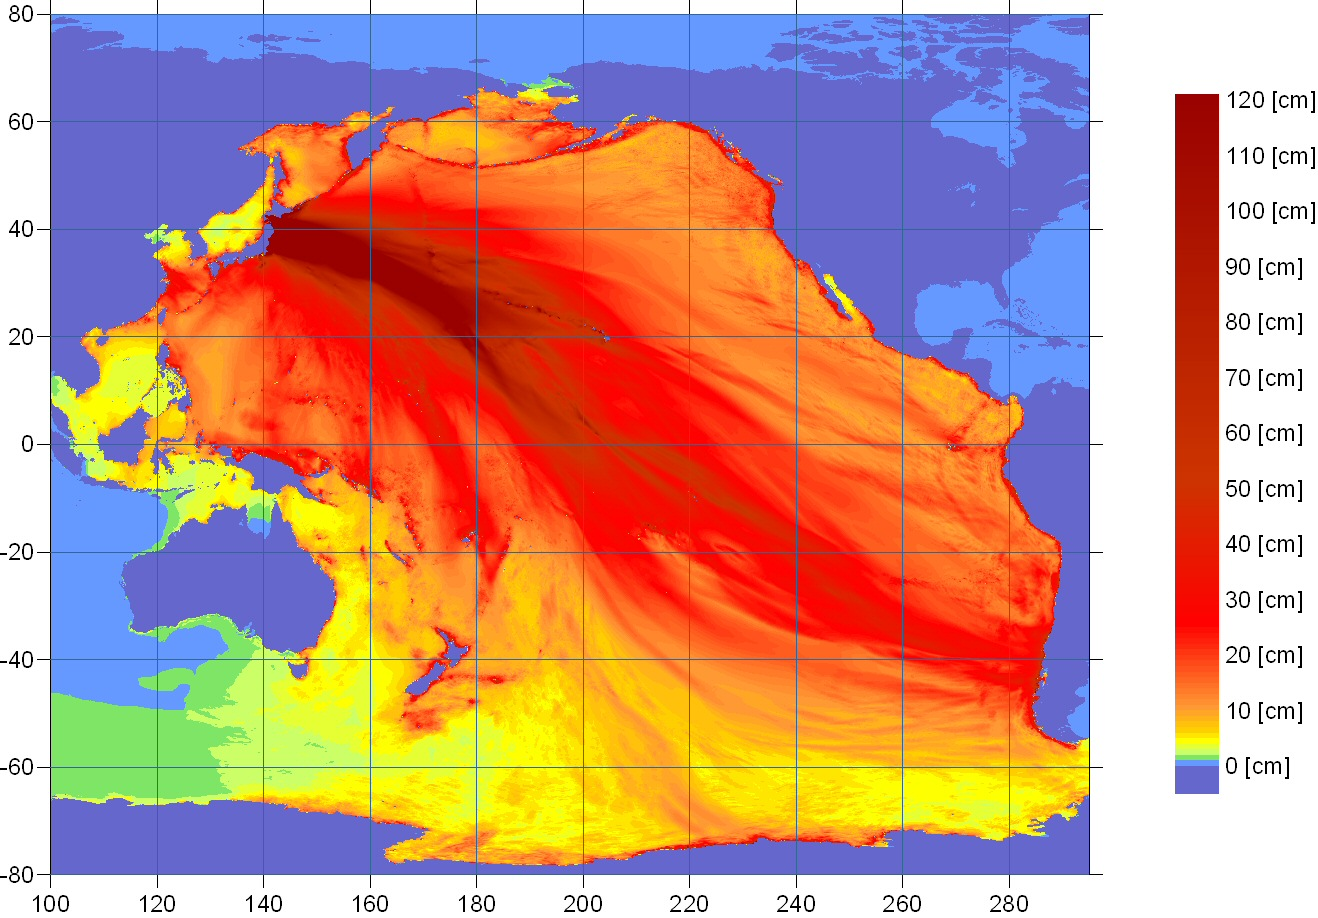
\includegraphics[width=\hsize]{graphics/sendaienergy}
\end{center}
\caption{Amplitude des Tsunami vom 11.~M"arz 2011.
Man beachte, dass durch die Wahl der Kartenprojektion 
die Grosskreise, entlang derer sich die Wellen ausbreiten,
zu S-Kurven gebogen werden. In K"ustenn"ahe nimmt die
Amplitude wegen der abnehmenden Wassertiefe und der damit
reduzierten Ausbreitungsgeschwindigkeit zu.
\label{tsunamienergie}}
\end{figure}


\subsection{Koordinaten und Randbedingungen}
Es interessieren uns nur die von einem Punkt aus erzeugte Wellen,
so wie dies bei einem Erdbeben der Fall ist. Die L"osung muss
notwendigerweise rotationssymmetrisch sein um eine Achse, die
durch den Ausgangspunkt verl"auft. 

Als Koordinatensystem auf einer Kugel verwenden wir Kugelkoordinaten
$(r,\vartheta,\varphi)$. $\vartheta$ ist die geographische Breite
vom Nordpol gemessen, der auch gleich der Ausgangspunkt der
Welle sein soll. $\varphi$ ist die geographische L"ange, wir
suchen jedoch eine L"osung, die von der geographischen Breite
unabh"angig ist. Ebenso interessiert uns der Radius $r$ nicht,
da wir uns auf die Kugeloberfl"ache beschr"anken wollen, wir
setzen daher $r=1$.

Gesucht ist also eine Funktion $u(t,\vartheta)$, welche die
Anfangsbedingungen
\begin{align*}
u(0,\vartheta)&=F(\vartheta)\\
\frac{\partial}{\partial t}u(0,\vartheta)&=G(\vartheta)
\end{align*}
erf"ullen m"ussen.

\subsection{Wellengleichung auf der Kugeloberfl"ache}
Die Wellengleichung auf der Kugeloberfl"ache entsteht als 
Einschr"ankung der dreidimensionalen Wellengleichung
$$
\frac1{c^2} \frac{\partial^2}{\partial t^2}u =\Delta u.
$$
Wir nehmen an, dass die Einheiten so gew"ahlt worden sind,
dass $c=1$ in diesen Einheiten gilt (dies erreicht man zum
Beispiel, wenn man als L"angeneinheit die in einer Zeiteinheit
zur"uckgelegte Strecke verwendet).
Der Laplace-Operator muss in Kugelkoordinaten ausgedr"uckt werden,
$$
\Delta u
=
\frac1{r^2} \frac{\partial}{\partial r}r^2\frac{\partial}{\partial r}u
+
\frac1{r^2\sin\vartheta}
\frac{\partial}{\partial\vartheta}
\sin\vartheta
\frac{\partial}{\partial\vartheta}
u
+
\frac1{r^2\sin^2\vartheta}\frac{\partial^2}{\partial\varphi^2}u
=
\frac1{\sin\vartheta}
\frac{\partial}{\partial\vartheta}
\sin\vartheta
\frac{\partial}{\partial\vartheta}
u
$$
Die Wellengleichung lautet jetzt also noch
\begin{equation}
\frac{\partial^2u}{\partial t^2}=
\frac1{\sin\vartheta}
\frac{\partial}{\partial\vartheta}
\sin\vartheta
\frac{\partial}{\partial\vartheta}
u=0.
\label{tsunami-gleichung}
\end{equation}

\subsection{Separation}
F"ur die L"osung der Wellengleichung (\ref{tsunami-gleichung}) machen
wir jetzt den "ublichen Separationsansatz:
$$
u(t,\vartheta)=T(t)\Theta(\vartheta),
$$
und setzen ihn in die Differentialgleichung ein:
$$
T''(t)\Theta(\vartheta)=
T(t)
\frac1{\sin\vartheta}
\frac{d}{d\vartheta}
\sin\vartheta
\frac{d}{d\vartheta}\Theta(\vartheta)
$$
Da wir eine L"osung suchen, die nicht "uberall verschwindet,
d"urfen wir annehmen, dass $T$ und $\Theta$ ausser an einzelnen
Punkten nicht verschwinden, dass wir also ``meistens'' durch
$T(t)\Theta(\vartheta)$ teilen d"urfen. Damit erreichen wir
die gew"unschte Trennung der Variablen:
\begin{equation}
\frac{T''(t)}{T(t)}
=
\frac1{\Theta(\vartheta)}
\frac1{\sin\vartheta}
\frac{d}{d\vartheta}
\sin\vartheta
\frac{d}{d\vartheta}\Theta(\vartheta)
\label{tsunami-separiert}
\end{equation}
Die linke Seite ist nur von $t$ abh"angig, die rechte nur von $\vartheta$,
diese Gleichung kann also nur erf"ullt sein, wenn beide seiten konstant
sind.  Wir erhalten also zwei Gleichungen
\begin{align}
T''(t)&=mT(t)
\label{tsunami:zeitabh}
\\
\frac1{\sin\vartheta}
\frac{d}{d\vartheta}
\sin\vartheta
\frac{d}{d\vartheta}\Theta(\vartheta)
&=m\Theta(\vartheta).
\label{tsunami:winkelabh}
\end{align}
Es ist jetzt also zu ermitteln, f"ur welche Werte von $m$ die beiden
Gleichungen L"osungen haben. Dann k"onnen f"ur diese Werte von $m$ 
L"osungen der partiellen Differentialgleichung zusammengebaut werden,
mit denen sich dann beliebige L"osungen durch "Uberlangerungen
erf"ullen lassen m"ussen.

\subsection{Zeitabh"angigkeit}
Die Zeitabh"angigkeit (\ref{tsunami:zeitabh}) ist eine gew"ohnliche
Schwingungsdifferentialgleichung.
Die L"osungen sollten Schwingungscharakter haben, was nur zutrifft, wenn
$m<0$ ist. Die allgemeine L"osung ist dann
\[
T_m(t)=a_m\cos\sqrt{-m}t+b_m\sin\sqrt{-m}t
\]

\subsection{Winkelabh"angigkeit}
Die Differentialgleichung (\ref{tsunami:winkelabh}) f"ur $\Theta$
ist in dieser Form etwas unhandlich.
Daher ersetzen wir $\Theta(\vartheta)$ durch eine
Funktion $y(x)$ mit Hilfe der Substitution $x=\cos\vartheta$.
Die Ableitung nach $\vartheta$ kann mit Hilfe der Kettenregel
in eine Ableitung nach $x$ umgewandelt werden:
\[
\frac{d}{d\vartheta}\Theta(\vartheta)
=\frac{dy(x)}{dx}\frac{dx}{d\vartheta}
=-\sin\vartheta \frac{d}{dx} y(x)
\]
Setzt man dies in die Differentialgleichung ein, wird sie zu
\begin{align*}
\frac1{\sin\vartheta}
(-\sin{\vartheta})\frac{d}{dx}\sin\vartheta (-\sin\vartheta)
\frac{d}{dx}y(x)
&=
\frac{d}{dx}\sin^2\vartheta\frac{d}{dx}y(x)\\
&=
\frac{d}{dx}(1-\cos^2\vartheta)\frac{d}{dx}y(x)\\
&=
\frac{d}{dx}(1-x^2)\frac{d}{dx}y(x).
\end{align*}
Die gesuchten Funktionen sind also L"osungen der Differentialgleichung
\begin{equation}
\frac{d}{dx}(1-x^2)\frac{d}{dx}y(x)
=
my(x)
\label{tsunamieigenwertproblem}
\end{equation}
Die Funktionen $y(x)$ m"ussen im ganzen Interval $[-1,1]$ definiert
sein. Dies ist nicht unbedingt selbstverst"andlich, wie schon der Fall
$m=0$ zeigt. In diesem Fall kann man die Differntialgleichung
durch zweimaliges Integrieren l"osen:
\begin{align*}
\frac{d}{dx}(1-x^2)\frac{d}{dx}y(x)&=0\\
(1-x^2)\frac{d}{dx}y(x)&=C\\
\frac{d}{dx}y(x)&=\frac{C}{1-x^2}\\
y(x)&=C\int\frac{dx}{1-x^2}\\
&=\frac{C}2\int\frac{dx}{1-x}+\frac{C}2\int\frac{dx}{1+x}\\
&=-\frac{C}2\log(1-x)+\frac{C}2\log(1+x) +D\\
&=\frac{C}2\log\frac{1+x}{1-x} + D
\end{align*}
An beiden Intervallenden w"achst die Funktion "uber alle Grenzen,
es sei denn es sei $C=0$.

Mit Sicherheit auf dem ganzen Interval definiert w"aren Polynome,
wir k"onnten also einen Ansatz
$$
y(x)=a_0+a_1+a_2x^2+\dots a_nx^n
$$
probieren. Setzt man dies in die Differentialgleichung ein und
beh"alt nur die Terme vom Grad $x^n$, bekommt man auf der rechten
Seite von (\ref{tsunamieigenwertproblem}) $ma_nx^n$, auf
der linken Seite
$$
-\frac{d}{dx}x^2\frac{d}{dx}a_nx^n
=
-\frac{d}{dx}x^2na_nx^{n-1}
=
-\frac{d}{dx}na_nx^{n+1}
=
-n(n+1)a_nx^n
$$
Damit folgt: $m=-n(n+1)$, nur f"ur solche Werte kann
(\ref{tsunamieigenwertproblem}) ein Polynom vom Grad $n$ als L"osung
haben. Die Differentialgleichung wird jetzt zu
\begin{equation}
\frac{d}{dx}(1-x^2)\frac{d}{dx}y(x)+n(n+1)y(x)=0
\label{legendredgl}
\end{equation}

\subsection{Legendre-Polynome}
Die Differentialgleichung (\ref{legendredgl}) ist die Differentialgleichung
der Legendre-Polynome.
Das Legendre-Polynom $P_n(x)$ ist eine polynomiale L"osung von
(\ref{legendredgl}) mit $P_n(1)=1$.
Dies legt aber die Funktion nicht fest, es sind weitere Bedingungen
n"otig. Daher wird verlangt, dass die Polynome auch orthogonal
sein sollen, also die Bedingung
$$
\int_{-1}^1 P_k(x)P_l(x)\,dx=0\quad\text{f"ur $k\ne l$}
$$
erf"ullen. Damit werden die Polynome eindeutig.
Die ersten sechs Legendre-Polynome sind
\begin{align*}
P_0(x)&=1\\
P_1(x)&=x\\
P_2(x)&=\frac12(3x^2-1)\\
P_3(x)&=\frac12(5x^3-3x)\\
P_4(x)&=\frac18(35x^4-30x^2+3)\\
P_5(x)&=\frac18(63x^5-70x^3+15x)
\end{align*}
Ausserdem gilt
$$
\int_{-1}^1 P_k(x)^2\,dx = \frac{2}{2k+1}.
$$
Da man 
jede Funktion auf dem Interval $[-1,1]$ mit Polynomen approximieren kann,
kann man auch jede Funktion durch Linearkombinationen von Legendre-Polynomen
$P_n(x)$ schreiben. 

Die Koeffizienten kann man mit Hilfe eines Integrals finden. Setzt man
$$
f(x)=\sum_{k\ge 0} c_k P_k(x)
$$
und berechnet man das Integral
$$
\int_{-1}^1 f(x)P_l(x)\,dx
=
\sum_{k\ge 0} c_k \int_{-1}^1 P_k(x)P_l(x)\,dx
=
\frac{2c_k}{2k+1}
$$
folgt
$$
c_k=\frac{2k+1}{2}\int_{-1}^1P_k(x)f(x)\,dx.
$$
Die Koeffizienten $c_k$ sind sozusagen die ``Legendre-Koeffizienten''
der Entwicklung der Funktion $f(x)$ nach Legendre-Polynomen.

\subsection{Anfangsbedingungen}
Unter Verwendung der Legendre-Polynome kann man jetzt die Wellengleichung
zu beliebigen Anfangsbedingungen l"osen.
Die L"osung der Differentialgleichung muss von der Form sein
$$
u(t, x)=\sum_{k=0}^{\infty}(a_k\cos \lambda_k t+b_k\sin\lambda_k t)P_k(x),
$$
wobei $\lambda_k=\sqrt{k(k+1)}$.
Die Koeffizienten m"ussen aus der Anfangsbedingung, also aus den 
Funktionen $F(\vartheta)=f(x)$ und $G(\vartheta)=g(x)$ bestimmt werden.
Die Anfangsbedingung f"ur $u(t,x)$ ergibt
\begin{align*}
u(0,x)
&=\sum_{k=0}^{\infty} a_kP_k(x)=f(x)
\end{align*}
F"ur $\partial_tu(t,x)$ ergibt sich entsprechend
\begin{align*}
\frac{\partial}{\partial t}u(0,x)
&=\sum_{k=0}^{\infty} \lambda_k b_kP_k(x)=g(x)
\end{align*}
Die Koeffizienten $a_k$ und $b_k$ kann man mit
\begin{align*}
a_k&=
\frac{2k+1}{2}\int_{-1}^1 P_k(x)f(x)\,dx
\\
b_k&=
\frac{2k+1}{2\lambda_k}\int_{-1}^1P_k(x)f(x)\,dx
\end{align*}
berechnen.

\subsection{Punktquelle}
\begin{figure}
\begin{center}
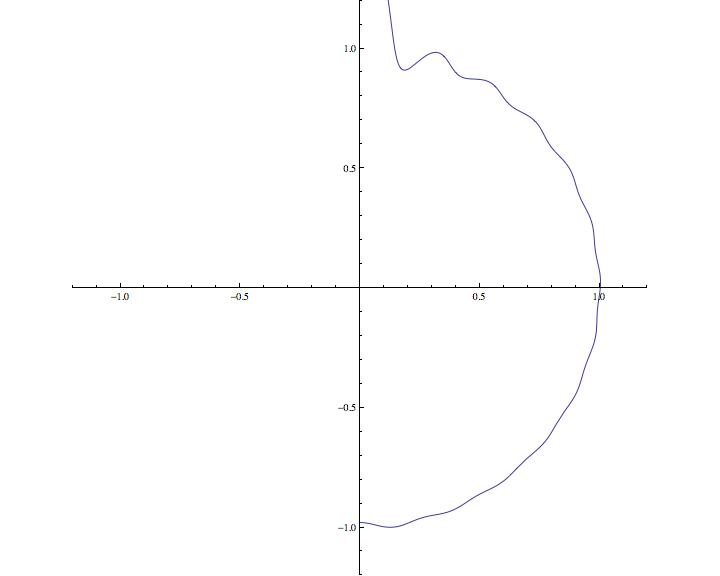
\includegraphics[width=\hsize]{graphics/tsunami0}
\end{center}
\caption{N"aherungsl"osung f"ur $N=25$ und $t=0$\label{tsunami0}}
\end{figure}
\begin{figure}
\begin{center}
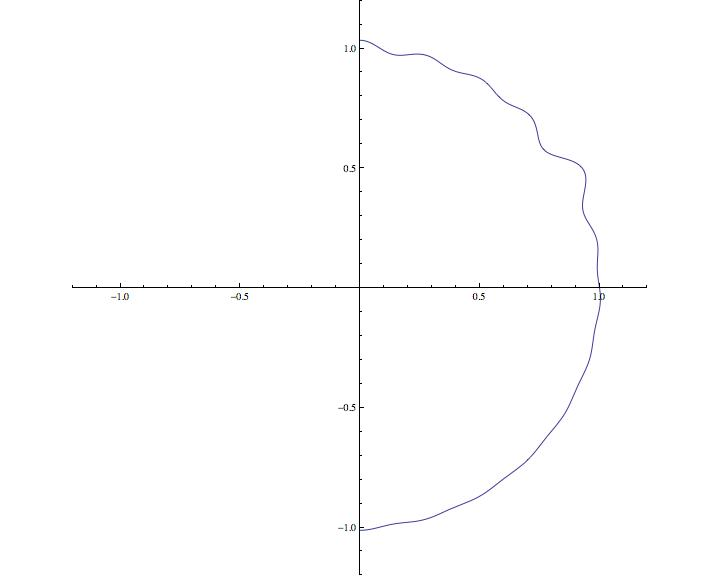
\includegraphics[width=\hsize]{graphics/tsunami50}
\end{center}
\caption{N"aherungsl"osung f"ur $N=25$ und $t=1$\label{tsunami50}}
\end{figure}



Wir w"ahlen jetzt eine spezielle Anfangsbedingung:
\begin{align*}
f_\varepsilon(x)&=\begin{cases}
\frac1{\varepsilon}&\qquad 1-\varepsilon<x\le 1\\
0&\qquad\text{sonst}
\end{cases}
\\
g(x)&=0
\end{align*}
In einer kleinen Umgebung des Nordpoles ist der Wert 
$\frac1{\varepsilon}$, also sehr gross, in allen anderen Punkten $0$.
Offenbar sind die $b_k=0$, und es bleiben nur die 
$a_k$ zu berechnen. Dazu gilt:
\begin{align*}
a_k(\varepsilon)&=\frac{2k+1}{2}\int_{-1}^1P_k(x)f_\varepsilon(x)\,dx
\\
&=\frac{2k+1}{2}\int_{1-\varepsilon}^1P_k(x)\frac1{\varepsilon}\,dx
\end{align*}
Da uns nur der Grenzwert $\varepsilon\to 0$ interessiert, gehen wir
zur Grenze "uber
\begin{align*}
\lim_{\varepsilon\to 0} a_k(\varepsilon)
&=
\frac{2k+1}{2}\lim_{\varepsilon\to 0}\frac1{\varepsilon}\int_{1-\varepsilon}^1P_k(x)\,dx
\end{align*}
Mit einer Stammfunktion $I_k(x)$ von $P_k(x)$ wird dies zu
\begin{align*}
\lim_{\varepsilon\to 0} a_k(\varepsilon)
&=
\frac{2k+1}{2}\lim_{\varepsilon\to 0}\frac{I_k(1)-I_k(1-\varepsilon)}{\varepsilon}
\\
&=\frac{2k+1}{2}I_k'(1)=\frac{2k+1}{2}P_k(1)=\frac{2k+1}{2}
\end{align*}
Als L"osung bekommt man damit formal
\begin{equation}
u(t,x)
=
\sum_{k=0}^\infty \frac{2k+1}{2}P_k(x) \cos \sqrt{k(k+1)}t.
\end{equation}
Leider ist diese Reihe nicht konvergent, was angesichts der sehr
speziellen Anfangsbedingungen auch nicht zu erwarten war.
Wenn man sie aber nach $N$ Termen abbricht, und mit $\frac1{N^2}$ 
normiert, erh"alt man eine L"osungsfunktion die ein ungef"ahres
Bild f"ur die Wellenausbreitung ergibt.
In den Abbildungen \ref{tsunami0} und \ref{tsunami50} wurde die Reihe nach 25 Termen
abgebrochen.
